%Wireframes
\section{Wireframes}

Here are all the views we plan to provide to the client for his website, we
add some explanations with an orange background to help you understanding
some parts of it. All of them are in French because it is one of the
client's requirement. But first, the next figure will show you how each wireframe is
linked to the others.

\begin{figure}[!ht]
    \centering
    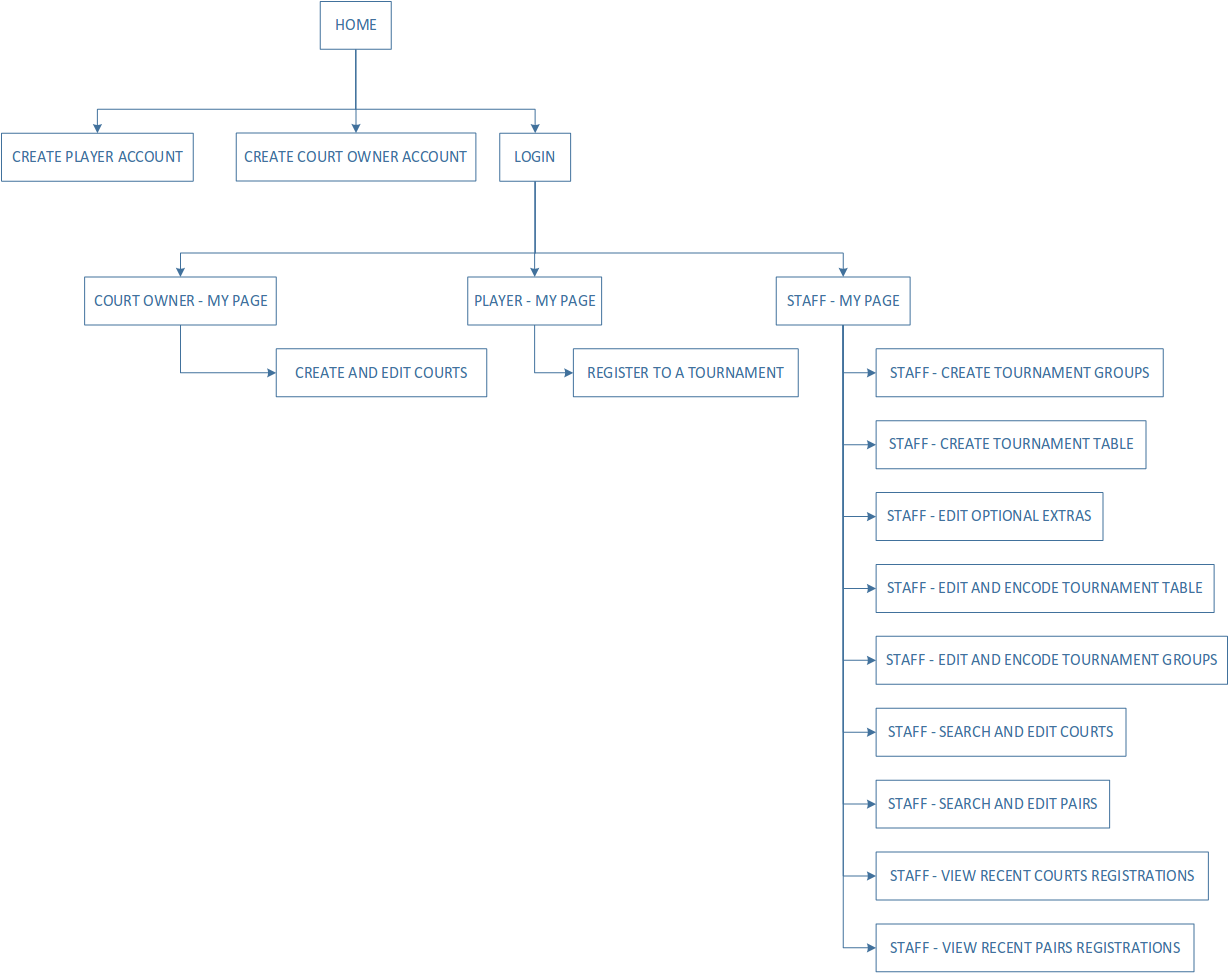
\includegraphics[width=\linewidth]{mockups-diagram.png}
    \caption{Wireframe diagram : explains how each wireframe is accessed}
\end{figure}
\FloatBarrier

\begin{figure}[!ht]
    \centering
    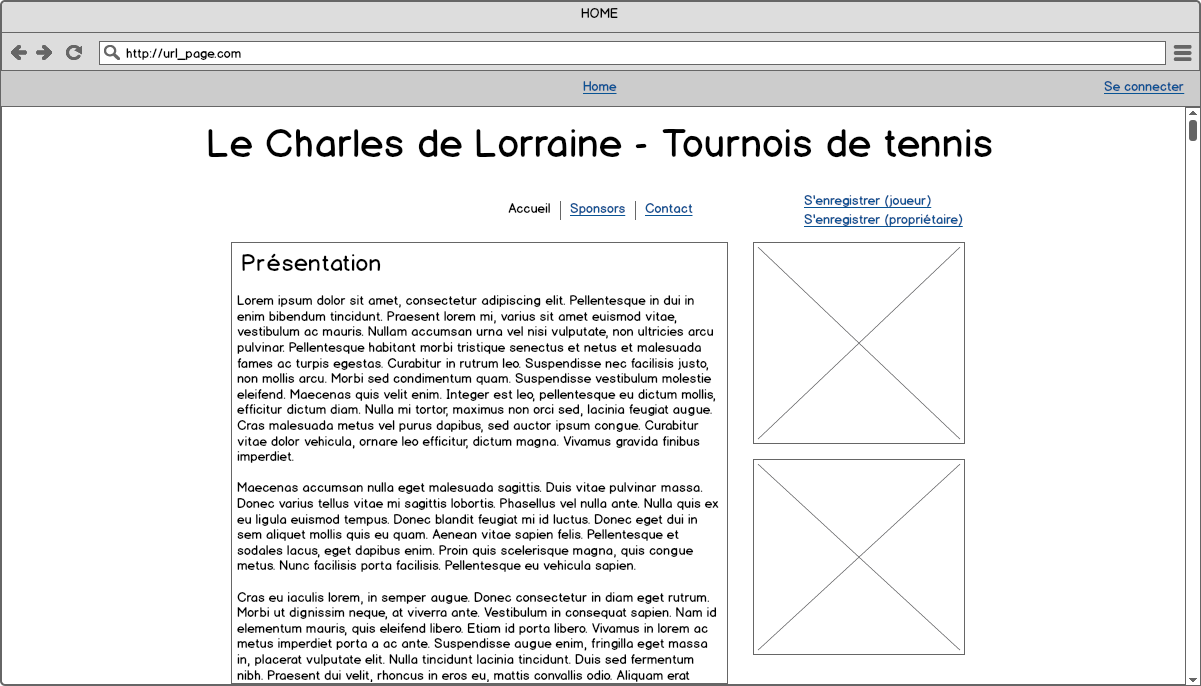
\includegraphics[width=\linewidth]{mockups/HOME.png}
    \caption{Wireframe : Home page}
\end{figure}
\FloatBarrier

\begin{figure}[!ht]
    \centering
    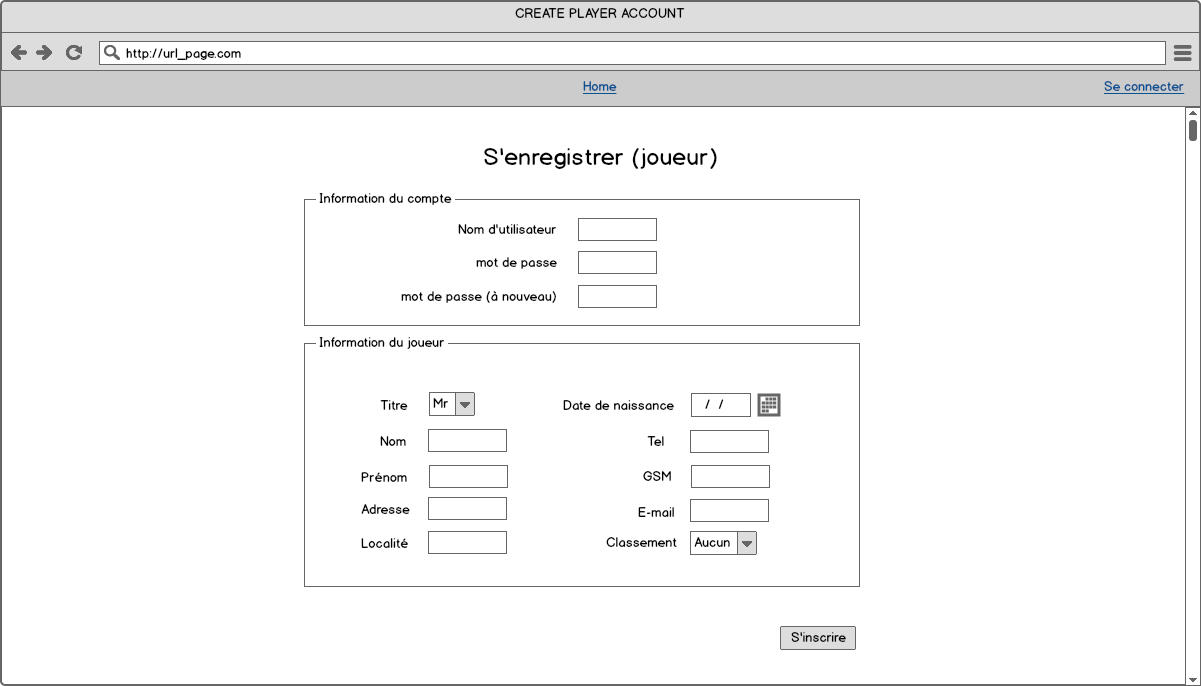
\includegraphics[width=\linewidth]{mockups/CREATE_PLAYER_ACCOUNT.png}
    \caption{Wireframe : Create player account}
\end{figure}
\FloatBarrier

\begin{figure}[!ht]
    \centering
    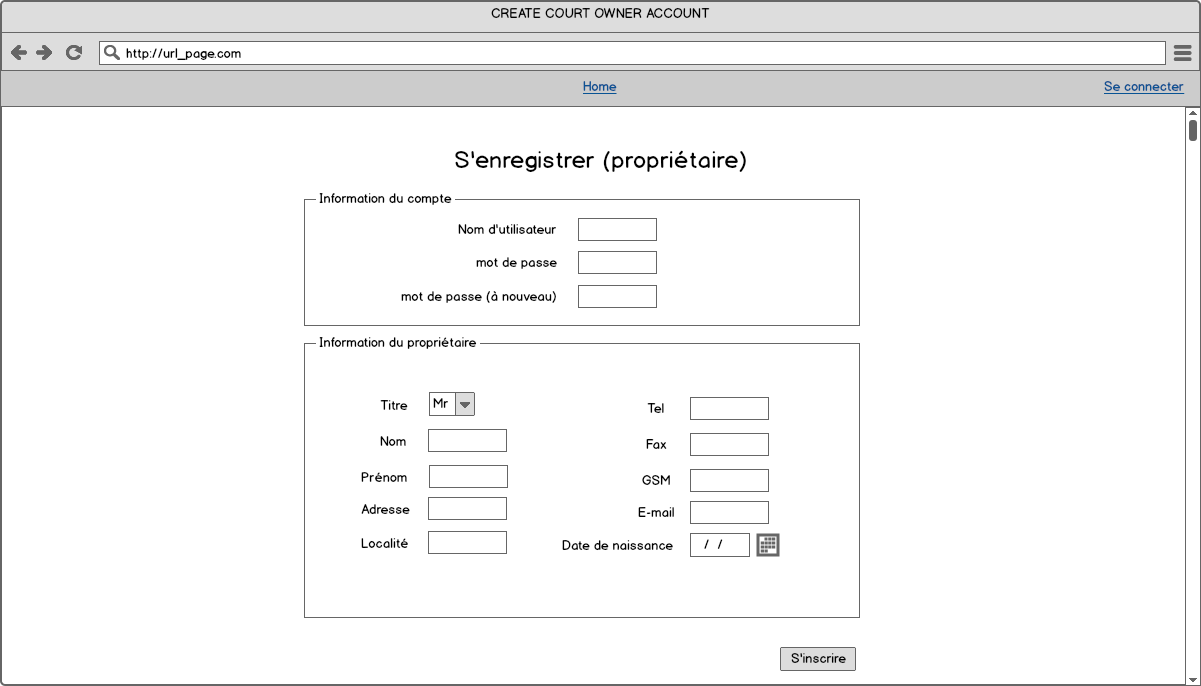
\includegraphics[width=\linewidth]{mockups/CREATE_COURT_OWNER_ACCOUNT.png}
    \caption{Wireframe : Create court owner account}
\end{figure}
\FloatBarrier

\begin{figure}[!ht]
    \centering
    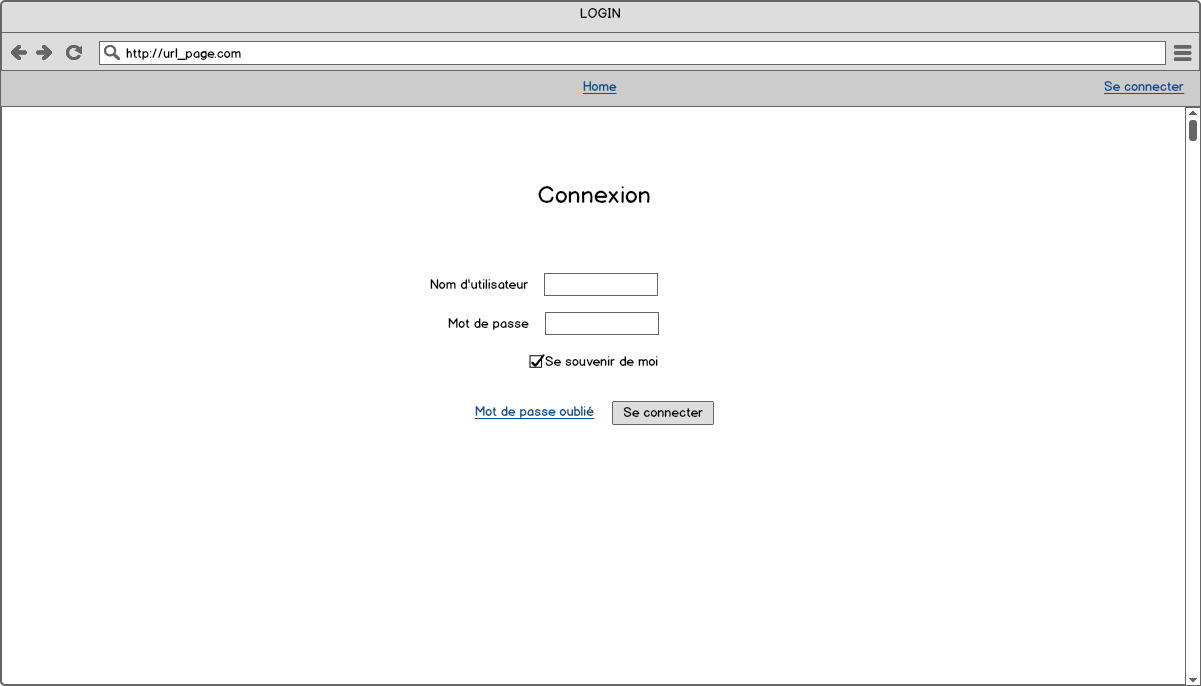
\includegraphics[width=\linewidth]{mockups/LOGIN.png}
    \caption{Wireframe : Login page}
\end{figure}
\FloatBarrier

\begin{figure}[!ht]
    \centering
    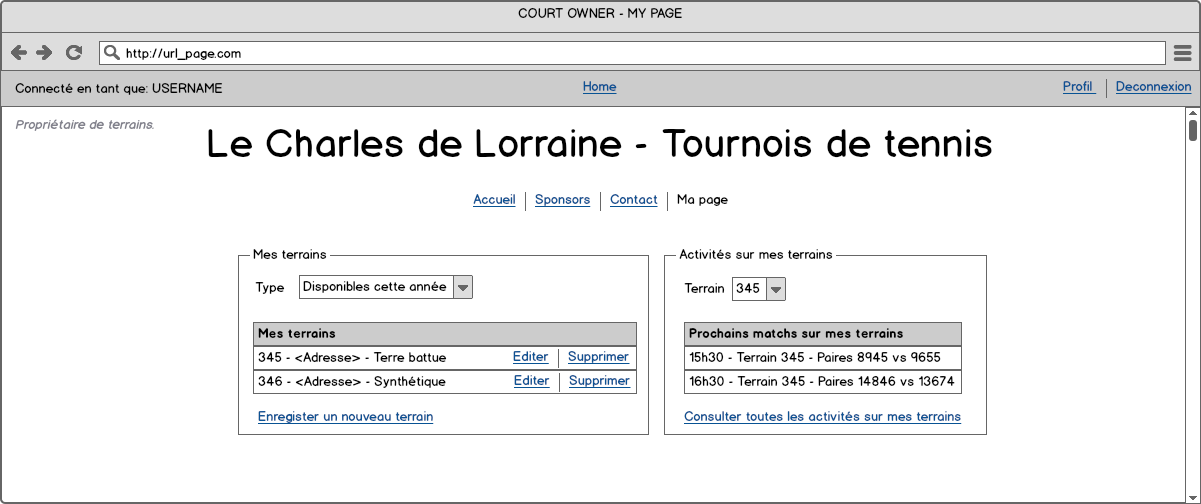
\includegraphics[width=\linewidth]{mockups/COURT_OWNER_-_MY_PAGE.png}
    \caption{Wireframe : Court owner - My page}
\end{figure}
\FloatBarrier

\begin{figure}[!ht]
    \centering
    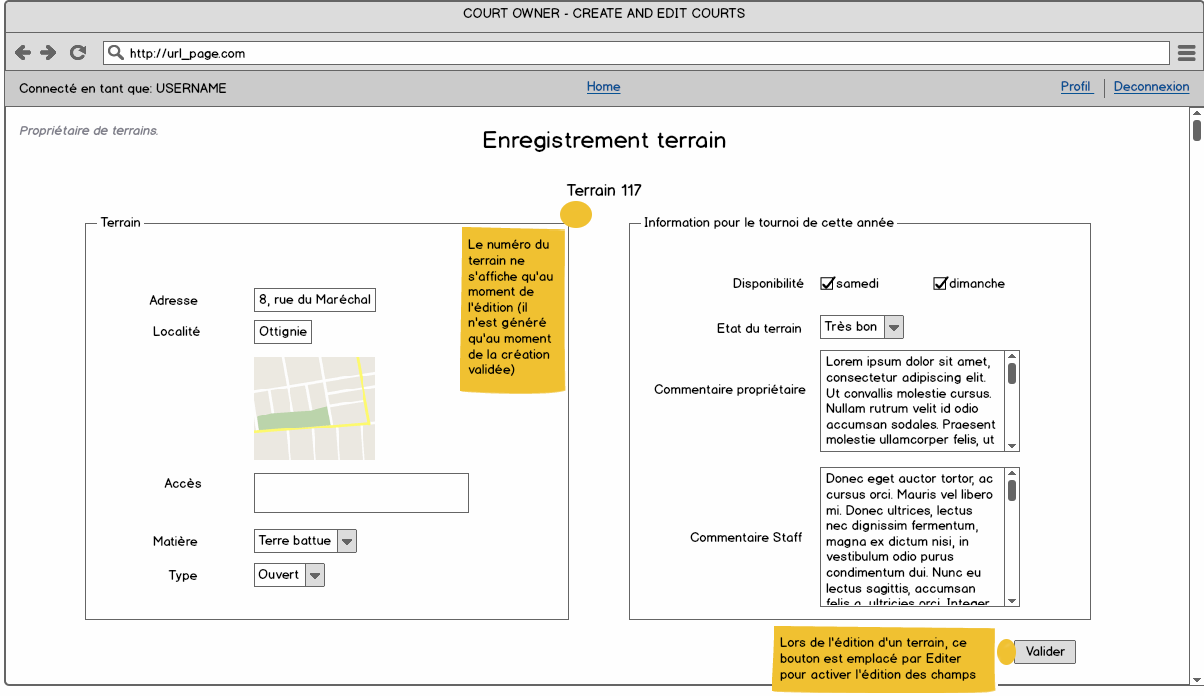
\includegraphics[width=1.1\linewidth]{mockups/COURT_OWNER_-_CREATE_AND_EDIT_COURT.png}
    \caption{Wireframe : Court owner - Create and edit court}
\end{figure}
\FloatBarrier

\begin{figure}[!ht]
    \centering
    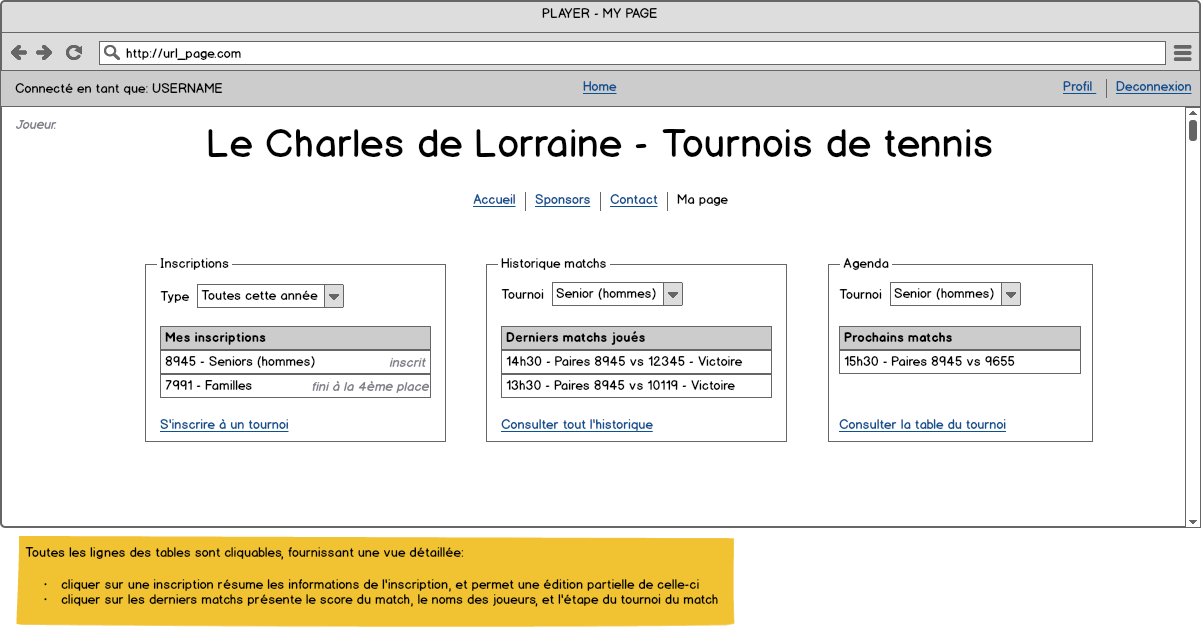
\includegraphics[width=\linewidth]{mockups/PLAYER_-_MY_PAGE.png}
    \caption{Wireframe : Player personal page}
\end{figure}
\FloatBarrier

\begin{figure}[!ht]
    \centering
    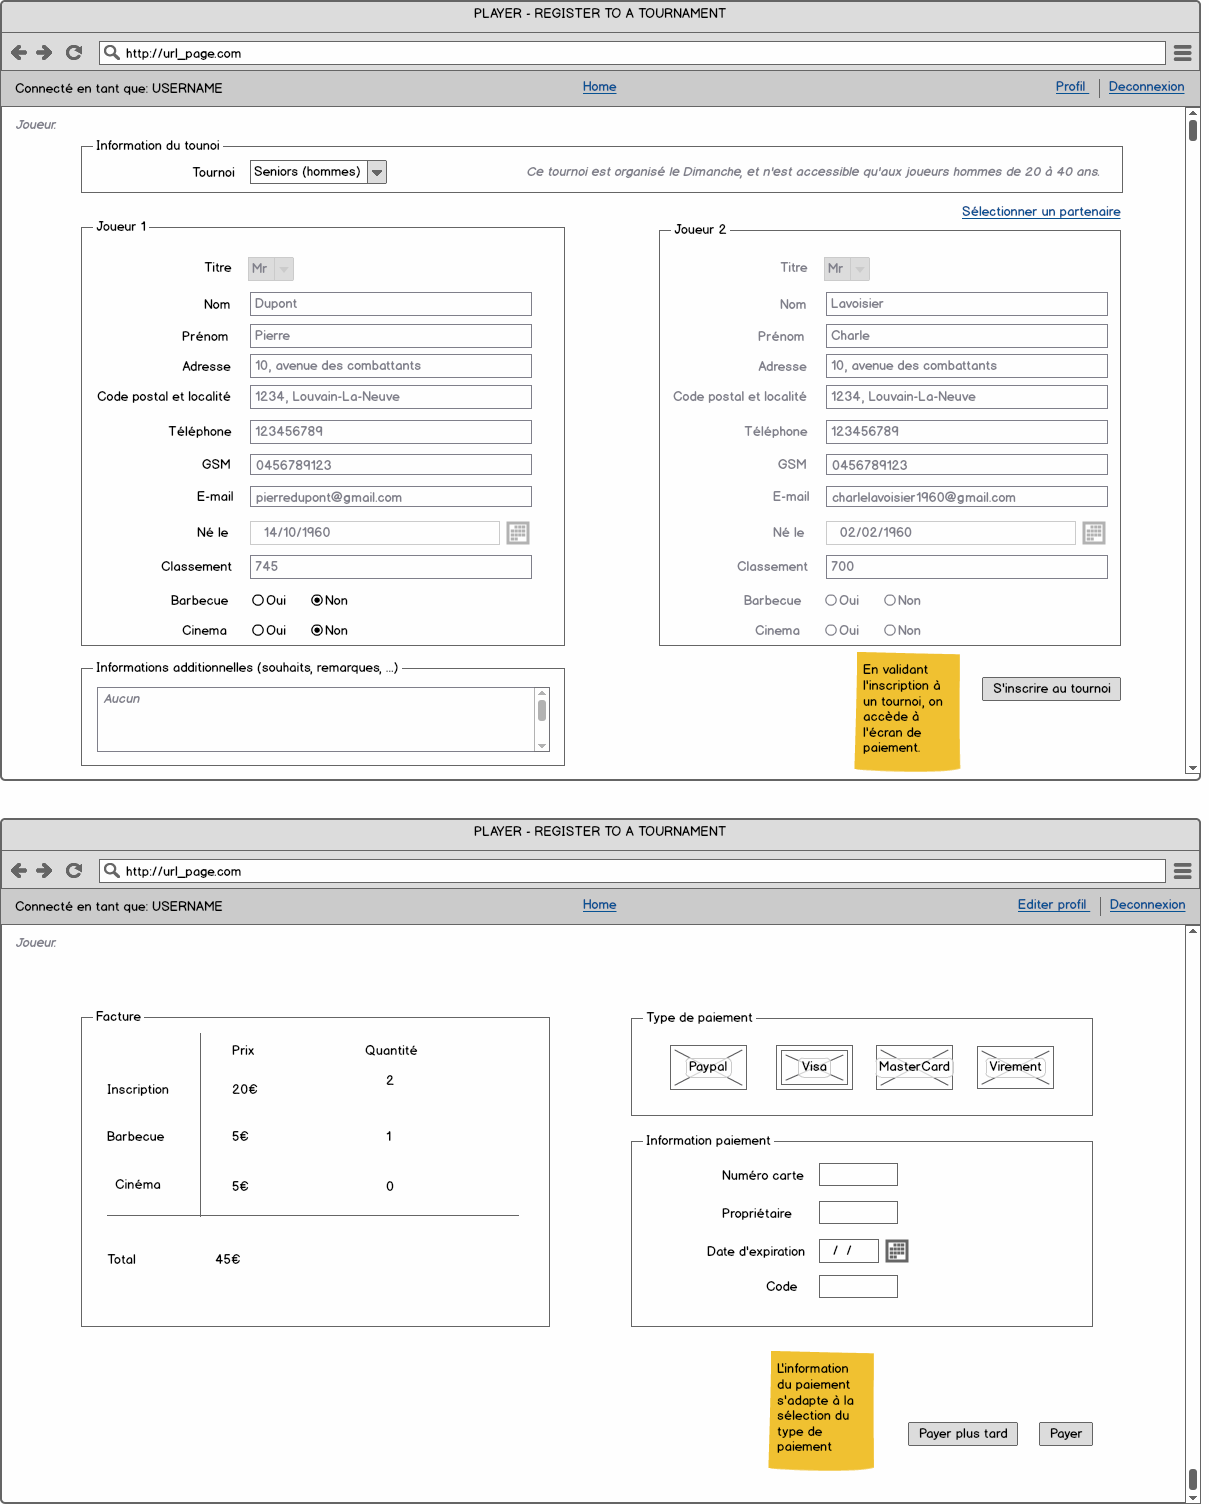
\includegraphics[width=\linewidth]{mockups/PLAYER_-_REGISTER_TO_A_TOURNAMENT.png}
    \caption{Wireframe : Player - Register to a tournament}
\end{figure}
\FloatBarrier

\begin{figure}[!ht]
    \centering
    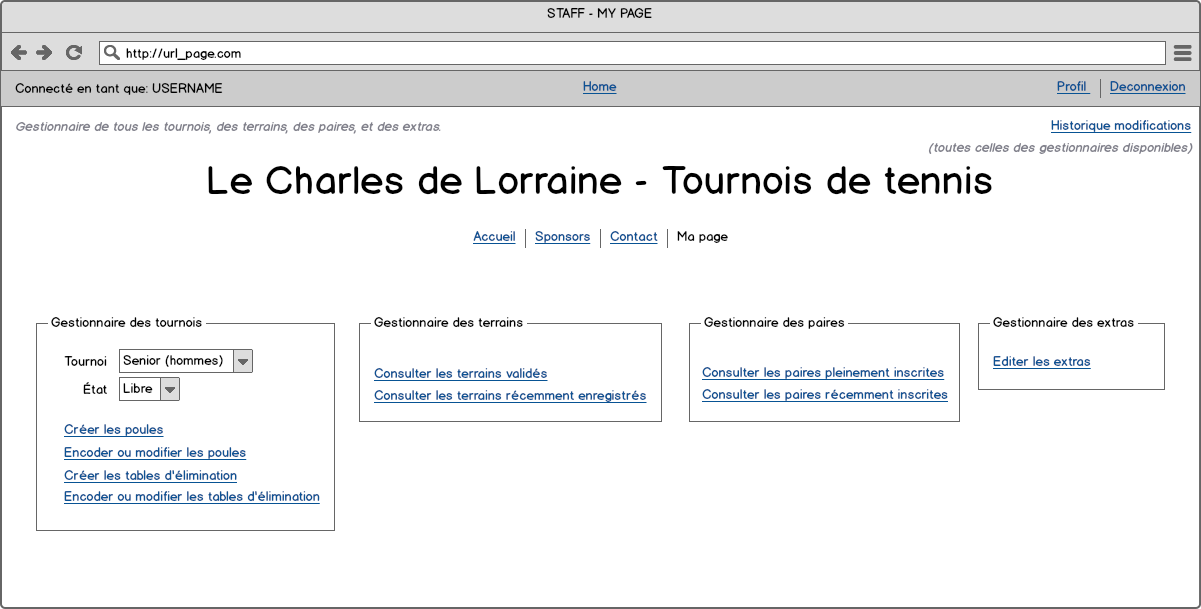
\includegraphics[width=\linewidth]{mockups/STAFF_-_MY_PAGE.png}
    \caption{Wireframe : Staff - personal page}
\end{figure}
\FloatBarrier

\begin{figure}[!ht]
    \centering
    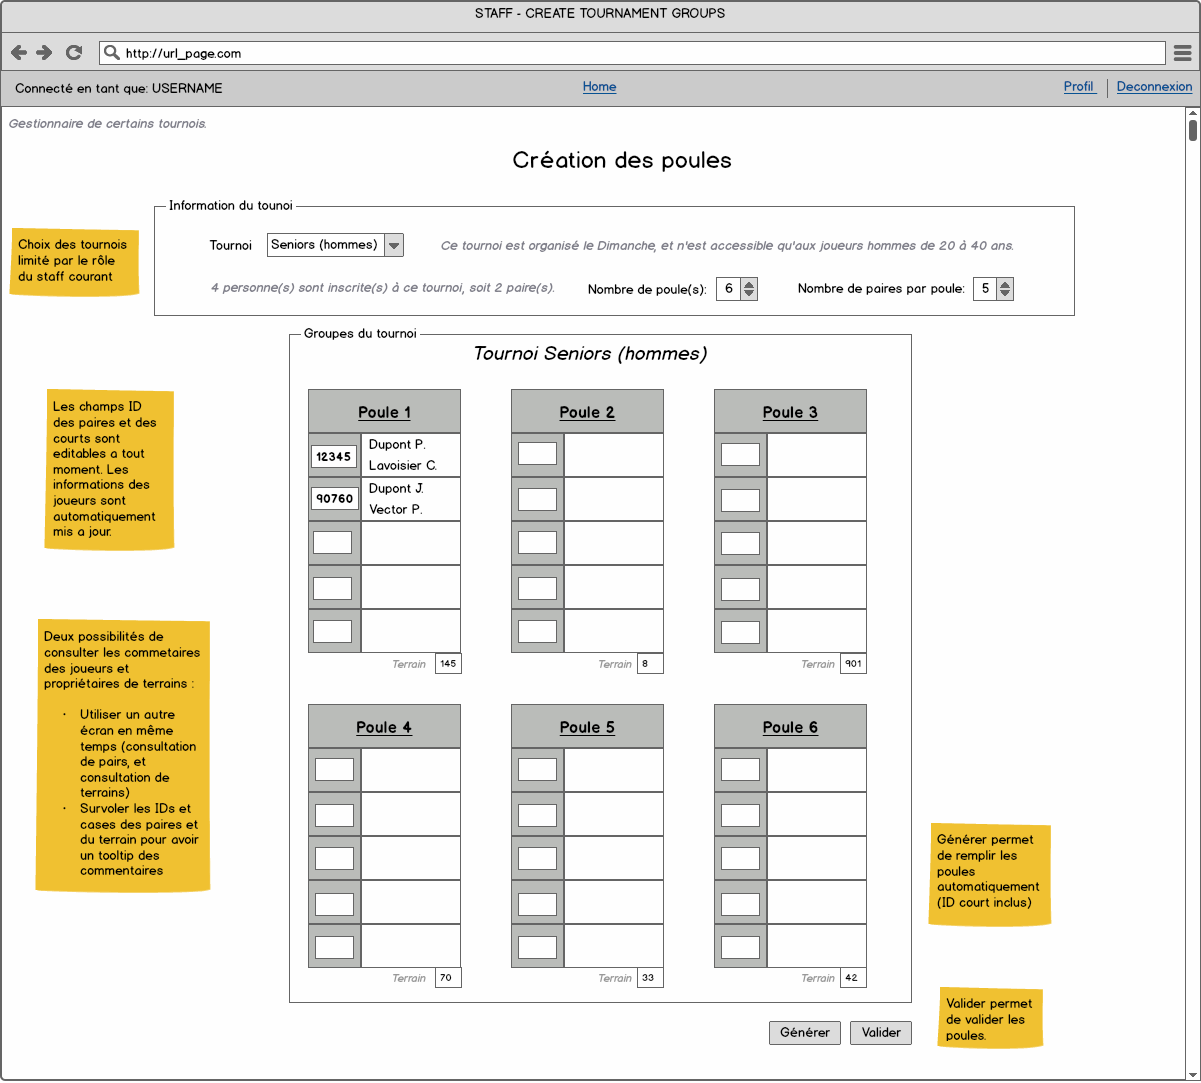
\includegraphics[width=\linewidth]{mockups/STAFF_-_CREATE_TOURNAMENT_GROUPS.png}
    \caption{Wireframe : Staff - Create tournament groups}
\end{figure}
\FloatBarrier

\begin{figure}[!ht]
    \centering
    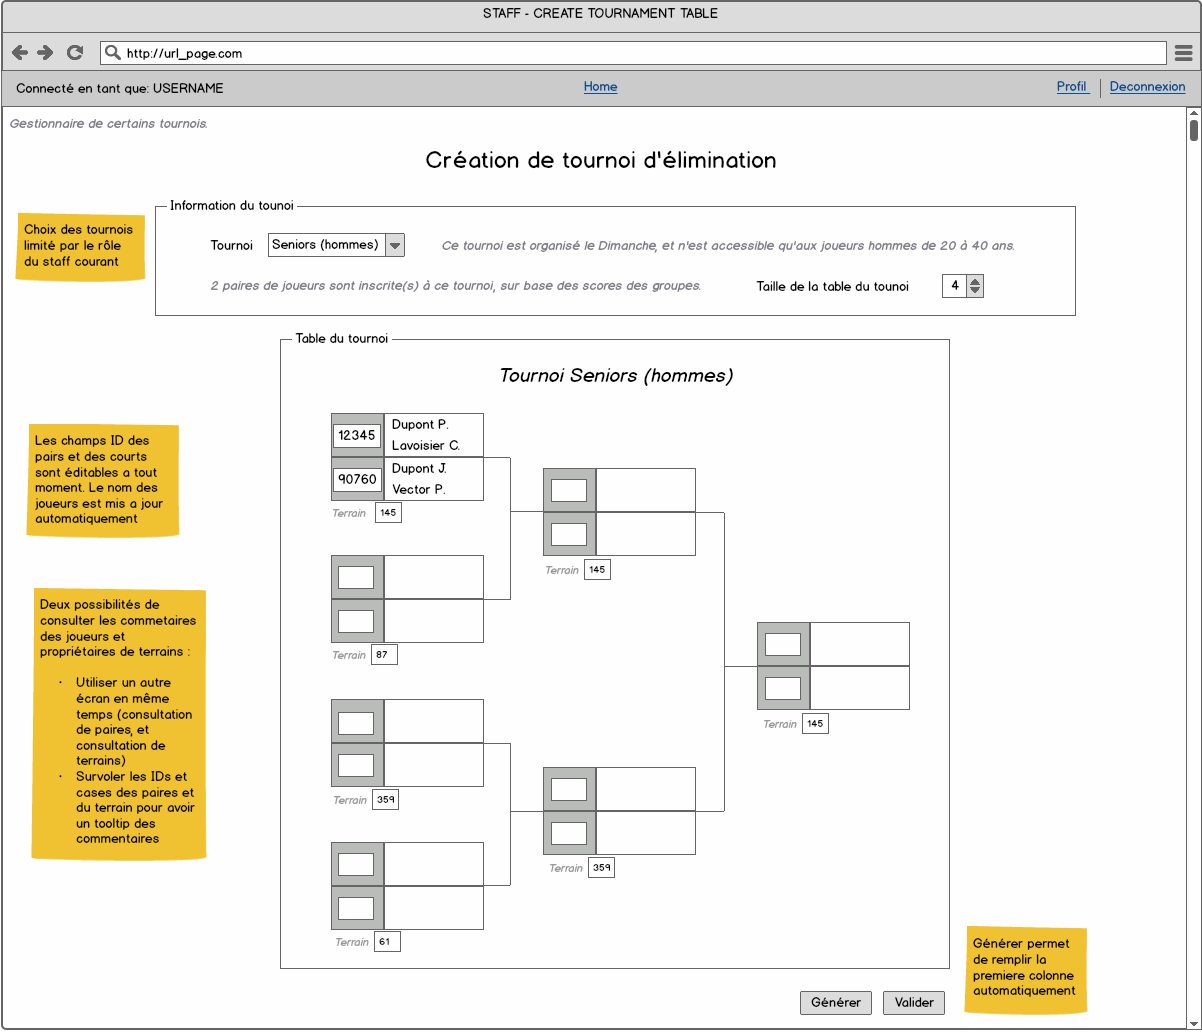
\includegraphics[width=\linewidth]{mockups/STAFF_-_CREATE_TOURNAMENT_TABLE.png}
    \caption{Wireframe : Staff - Create tournament table}
\end{figure}
\FloatBarrier

\begin{figure}[!ht]
    \centering
    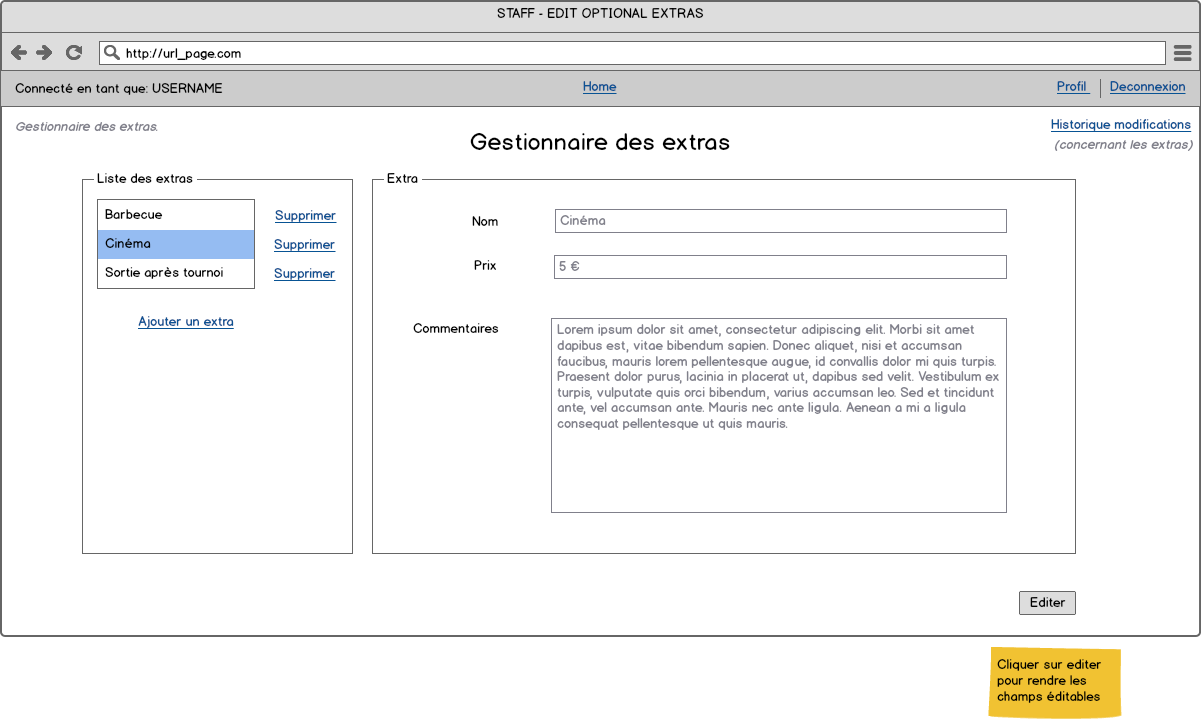
\includegraphics[width=\linewidth]{mockups/STAFF_-_EDIT_OPTIONAL_EXTRAS.png}
    \caption{Wireframe : Staff - Edit optional extras}
\end{figure}
\FloatBarrier

\begin{figure}[!ht]
    \centering
    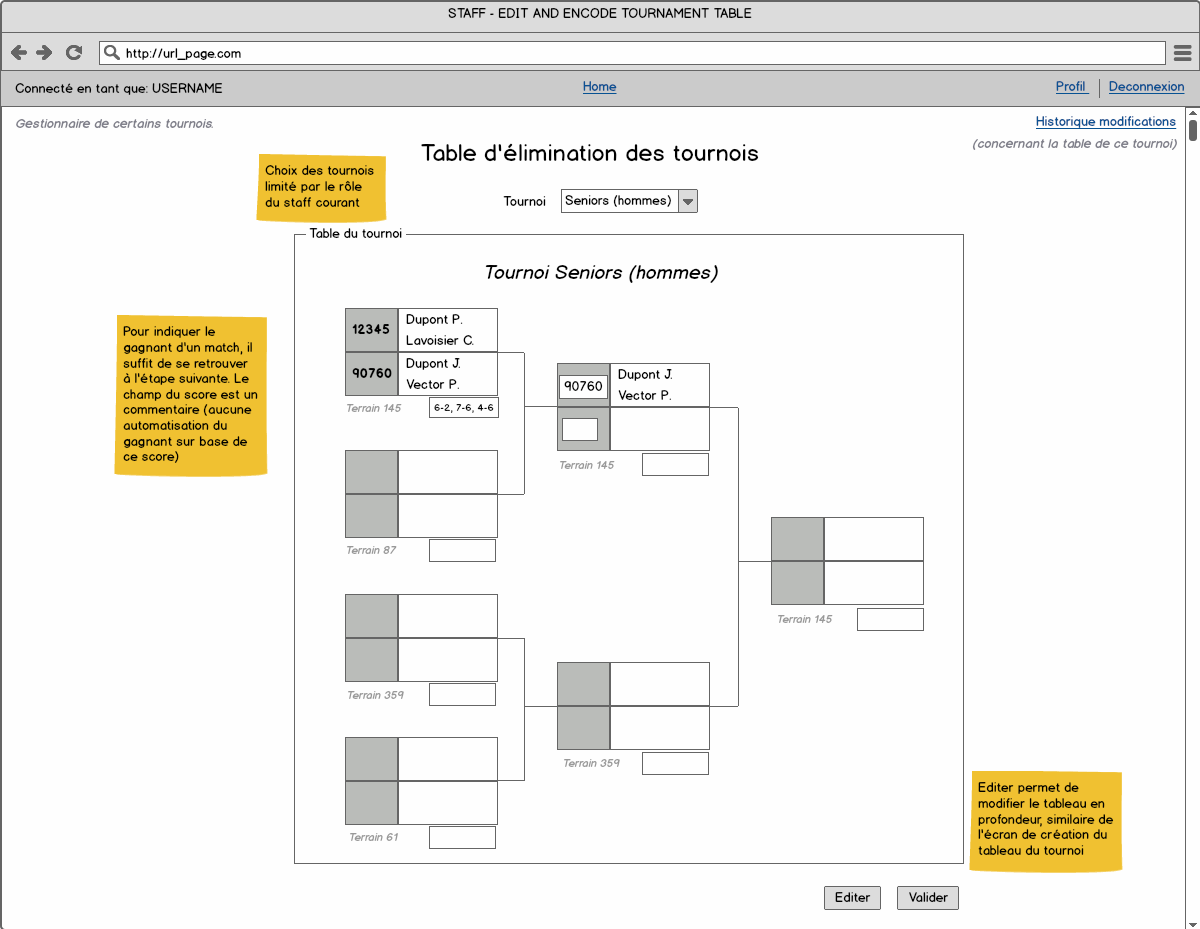
\includegraphics[width=\linewidth]{mockups/STAFF_-_EDIT_AND_ENCODE_TOURNAMENT_TABLE.png}
    \caption{Wireframe : Staff - Edit and encode tournament table}
\end{figure}
\FloatBarrier

\begin{figure}[!ht]
    \centering
    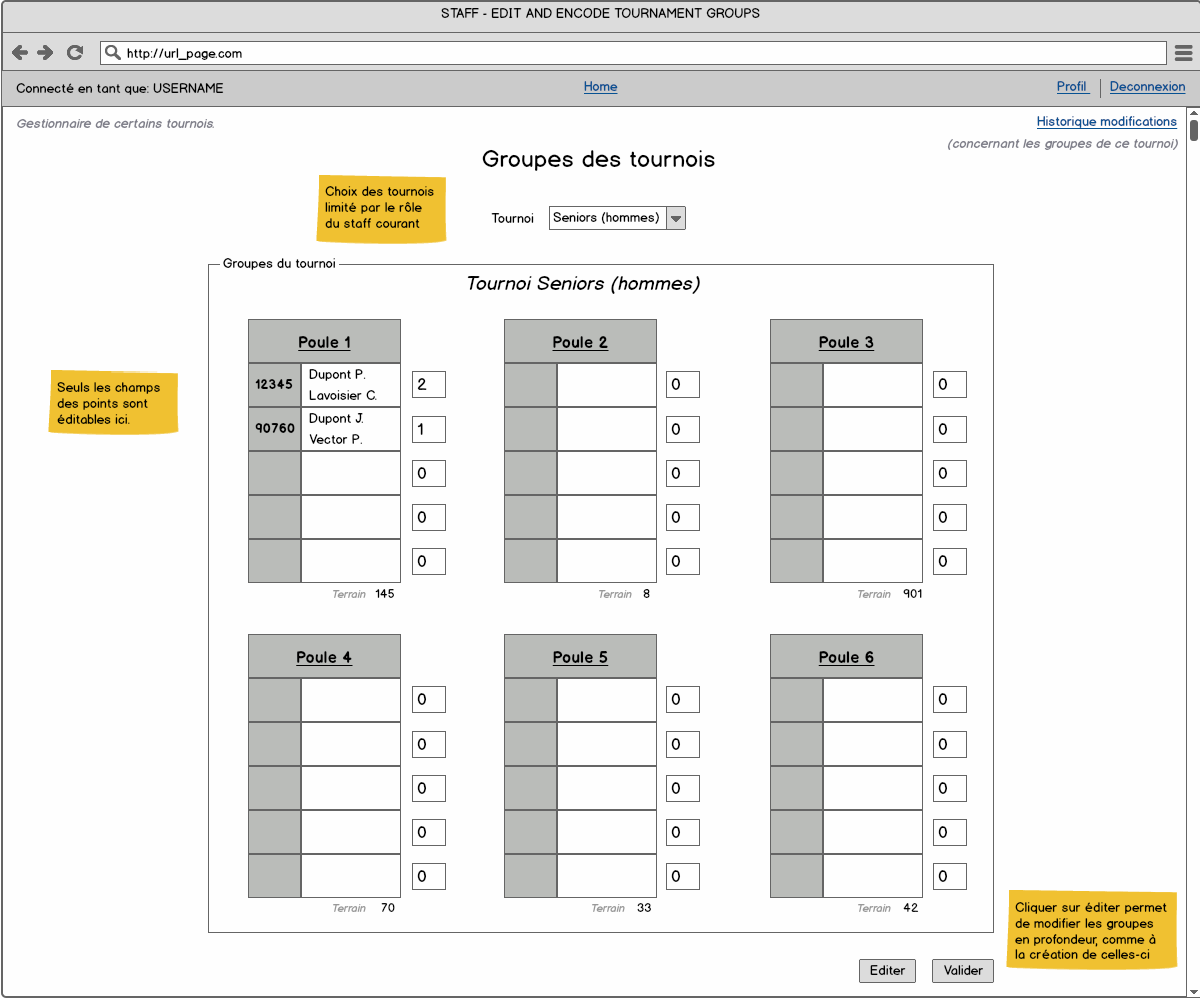
\includegraphics[width=\linewidth]{mockups/STAFF_-_EDIT_AND_ENCODE_TOURNAMENT_GROUPS.png}
    \caption{Wireframe : Staff - Edit and encode tournament groups}
\end{figure}
\FloatBarrier

\begin{figure}[!ht]
    \centering
    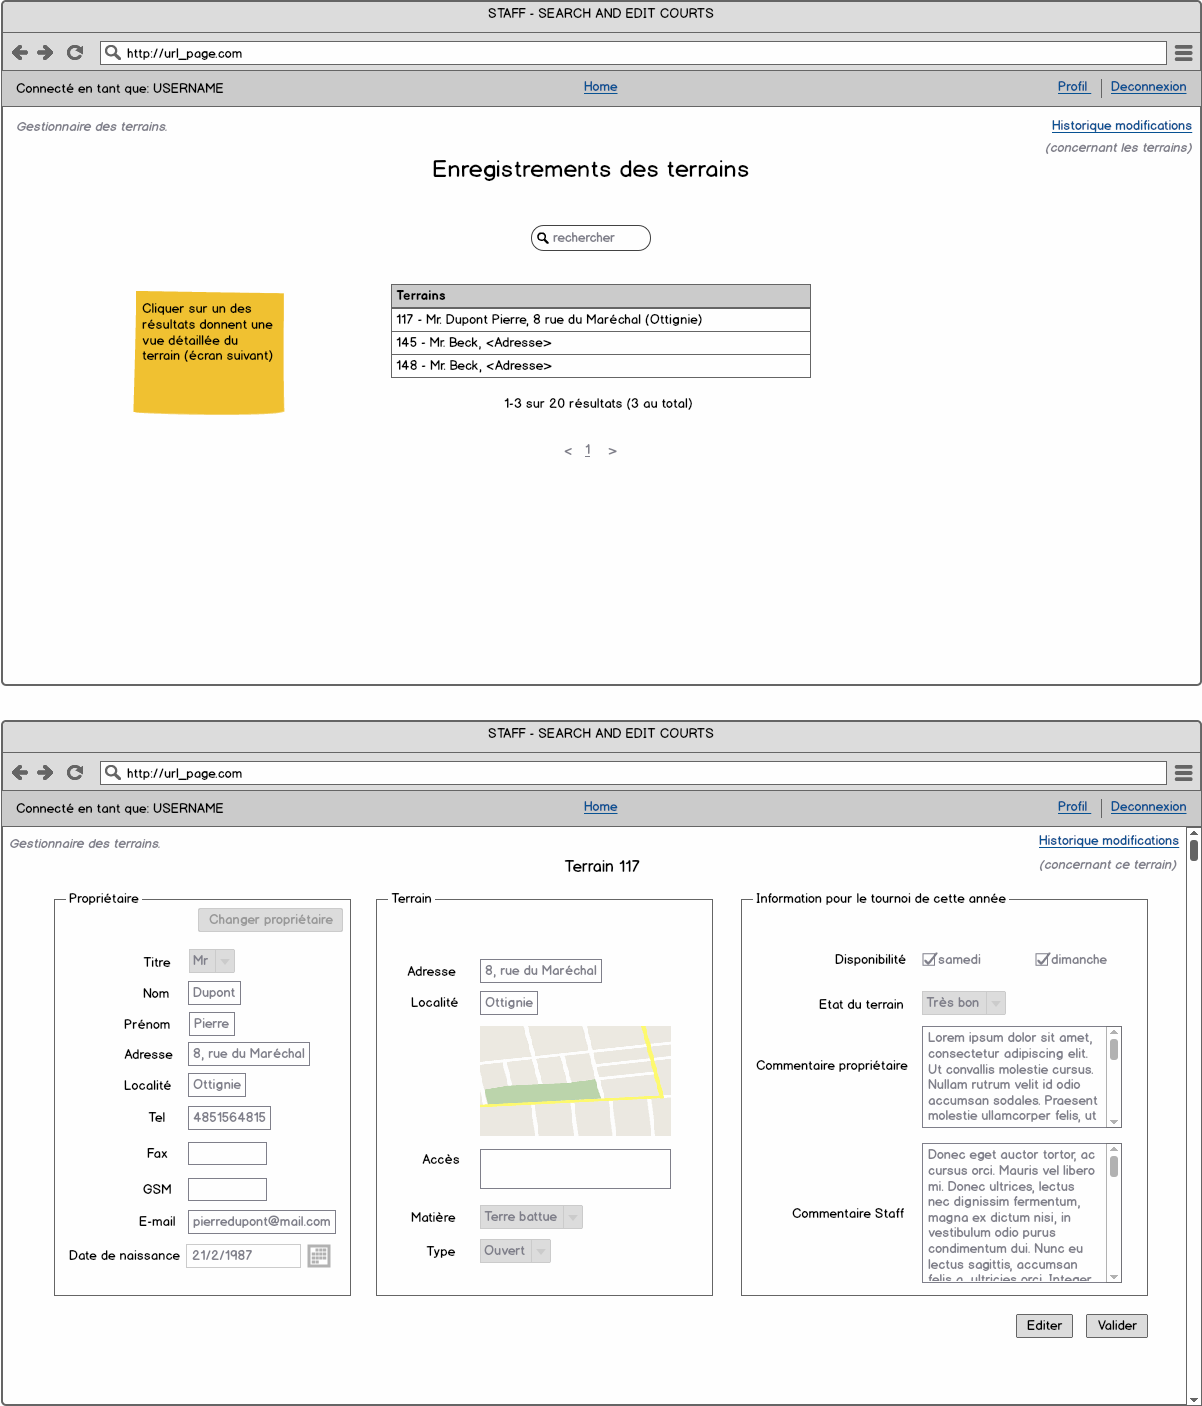
\includegraphics[width=\linewidth]{mockups/STAFF_-_SEARCH_AND_EDIT_COURTS.png}
    \caption{Wireframe : Staff - Search and edit courts}
\end{figure}
\FloatBarrier

\begin{figure}[!ht]
    \centering
    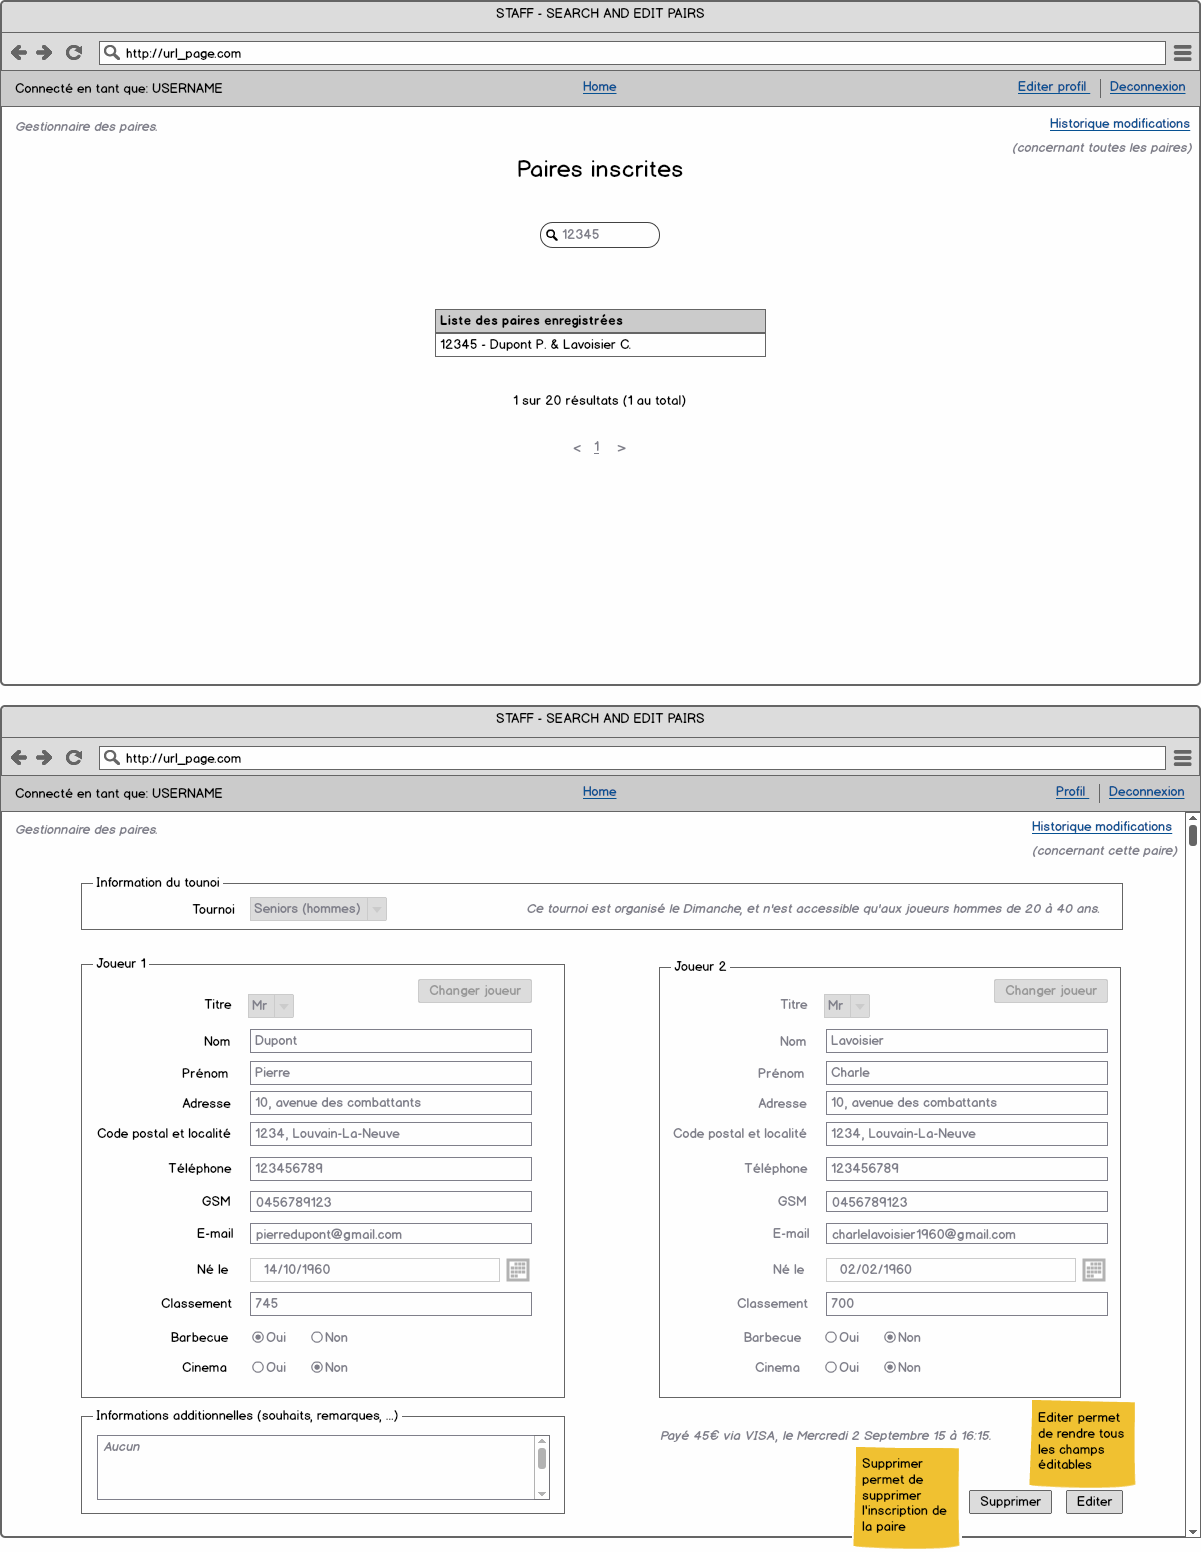
\includegraphics[width=\linewidth]{mockups/STAFF_-_SEARCH_AND_EDIT_PAIRS.png}
    \caption{Wireframe : Staff - Search and edit pairs}
\end{figure}
\FloatBarrier

\begin{figure}[!ht]
    \centering
    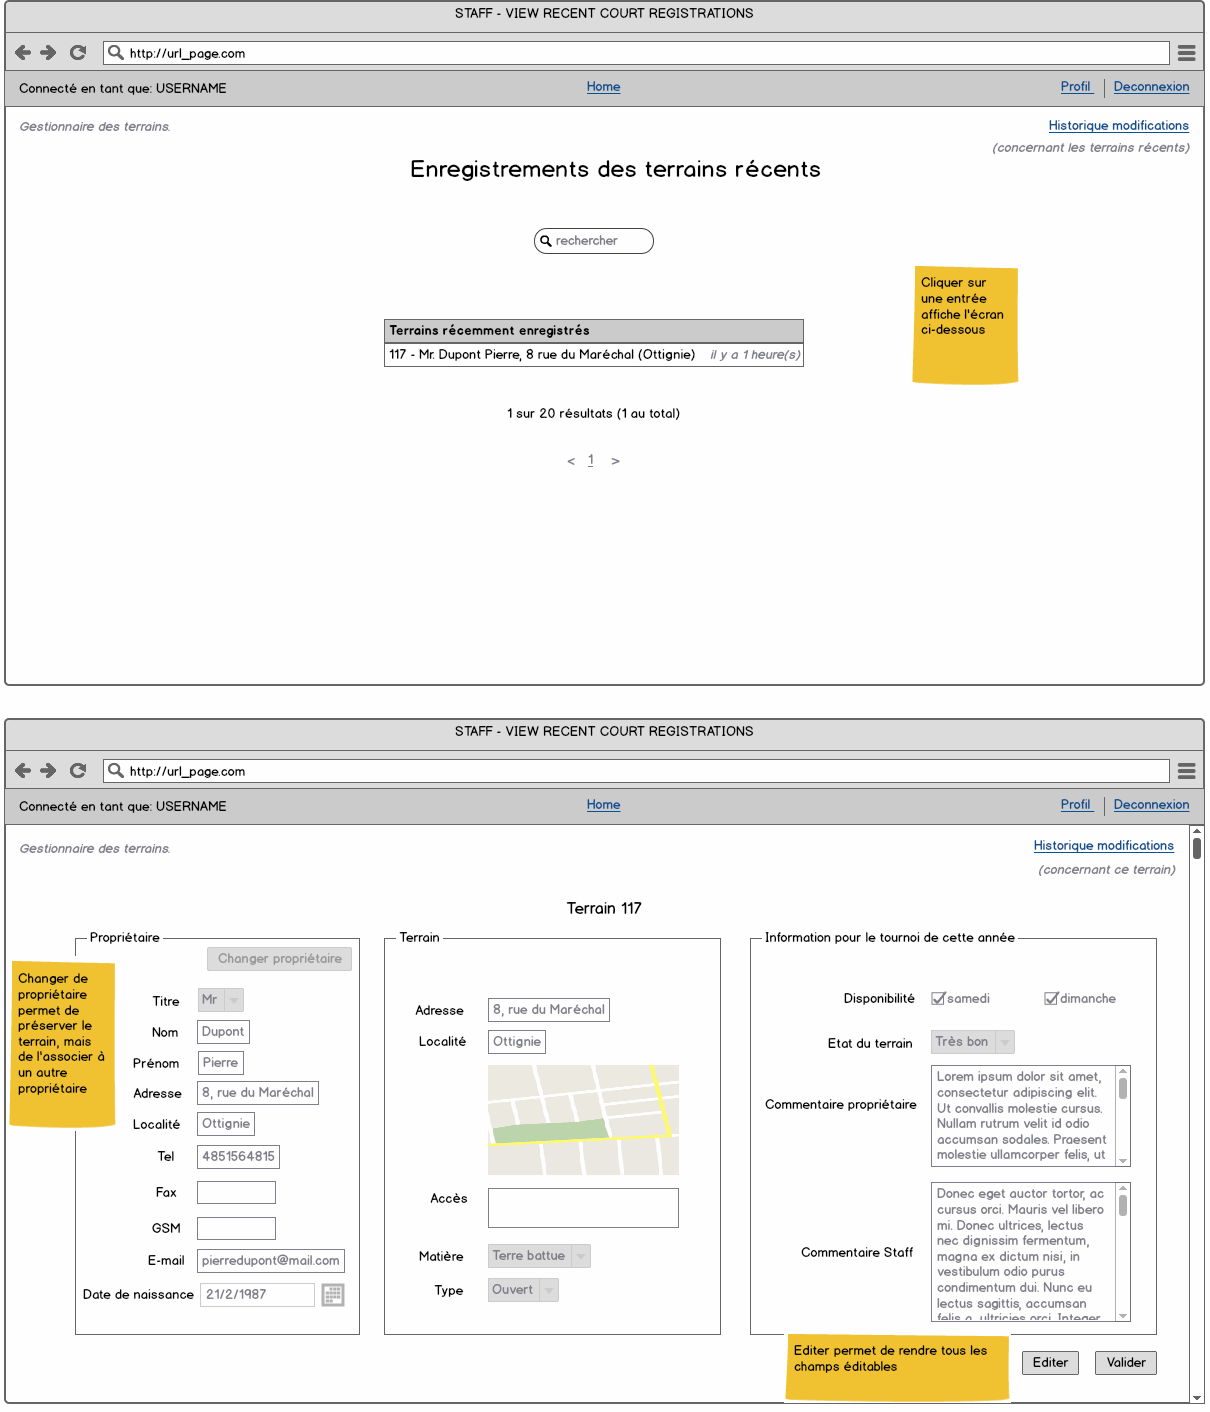
\includegraphics[width=\linewidth]{mockups/STAFF_-_VIEW_RECENT_COURTS_REGISTRATION.png}
    \caption{Wireframe : Staff - View recent courts registration}
\end{figure}
\FloatBarrier

\begin{figure}[!ht]
    \centering
    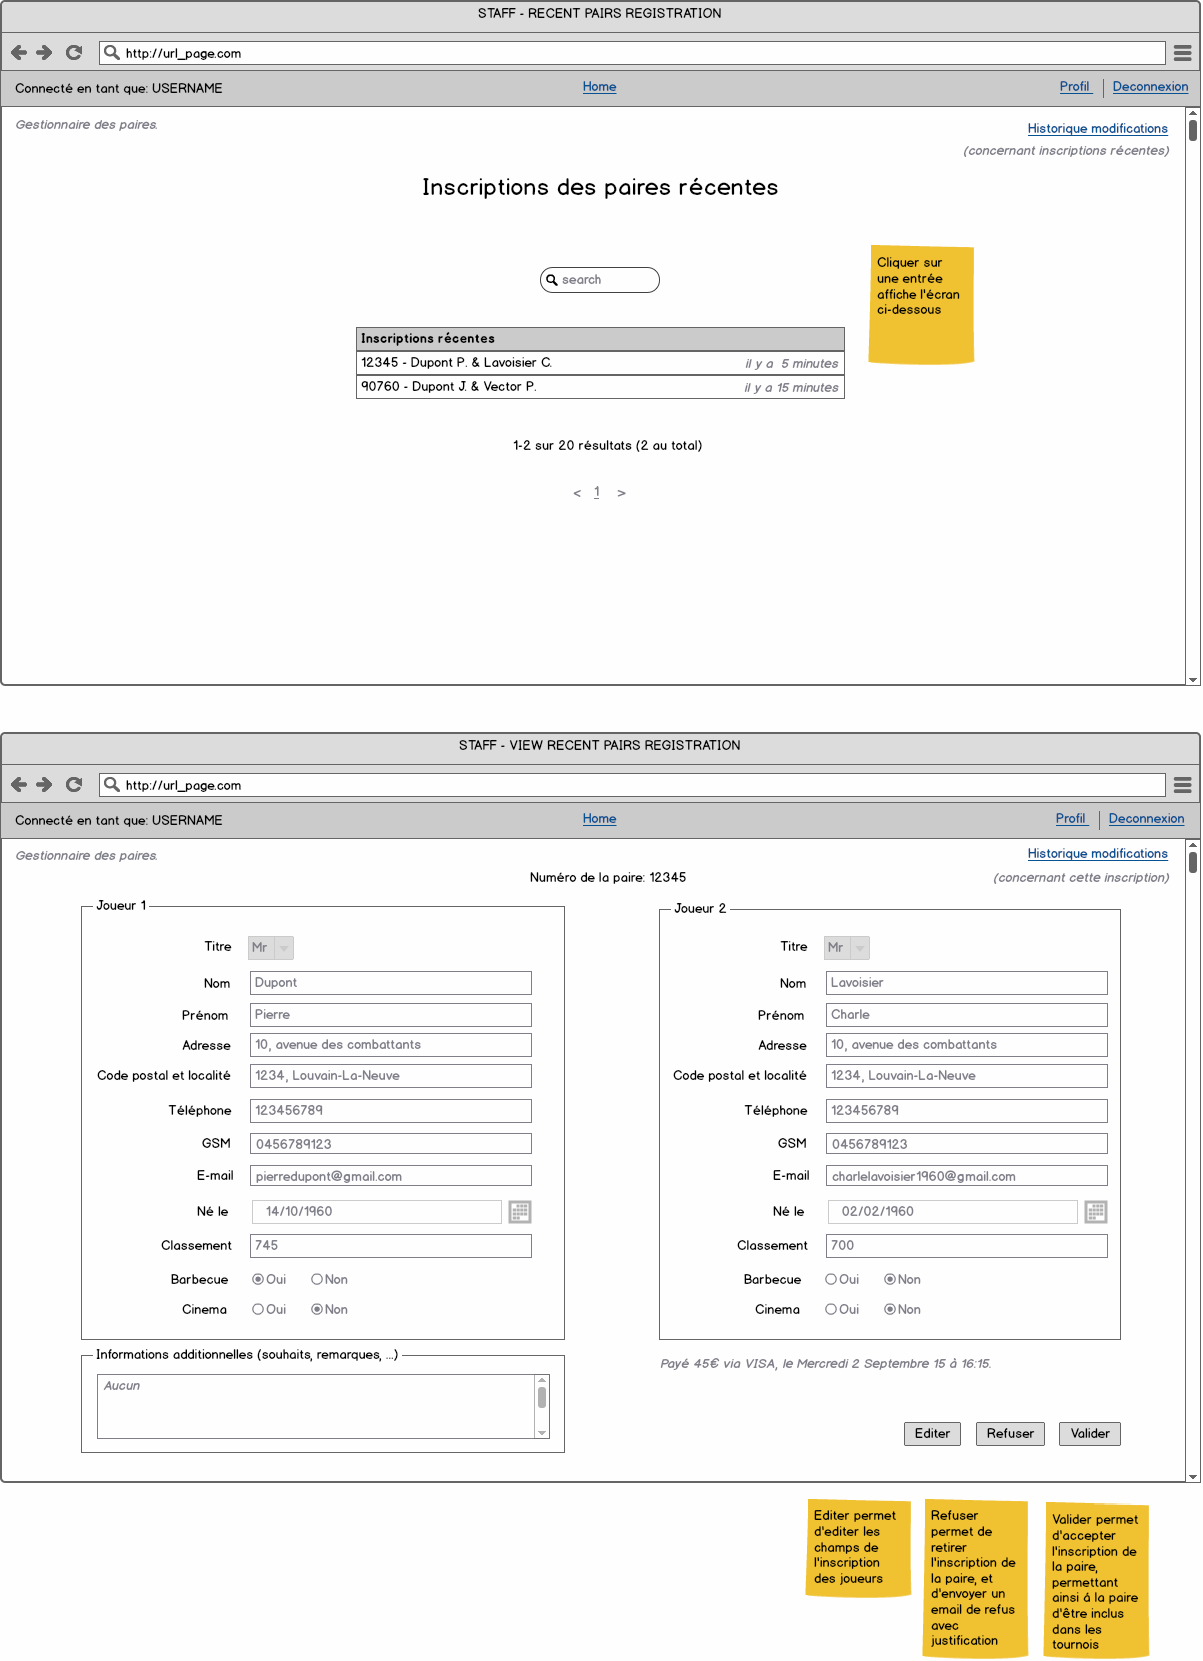
\includegraphics[width=\linewidth]{mockups/STAFF_-_VIEW_RECENT_PAIRS_REGISTRATION.png}
    \caption{Wireframe : Staff - View recent pairs registration}
\end{figure}
\FloatBarrier

